%%%%%%%%%%%%%%%%%%%%%%%%%%%%%%%%%%%%%%%%%
% Beamer Presentation
% LaTeX Template
% Version 1.0 (10/11/12)
%
% This template has been downloaded from:
% http://www.LaTeXTemplates.com
%
% License:
% CC BY-NC-SA 3.0 (http://creativecommons.org/licenses/by-nc-sa/3.0/)
%
%%%%%%%%%%%%%%%%%%%%%%%%%%%%%%%%%%%%%%%%%

%----------------------------------------------------------------------------------------
%	PACKAGES AND THEMES
%----------------------------------------------------------------------------------------

\documentclass{beamer}

\mode<presentation> {

% The Beamer class comes with a number of default slide themes
% which change the colors and layouts of slides. Below this is a list
% of all the themes, uncomment each in turn to see what they look like.

%\usetheme{default}
%\usetheme{AnnArbor}
%\usetheme{Antibes}
%\usetheme{Bergen}
%\usetheme{Berkeley}
%\usetheme{Berlin}
%\usetheme{Boadilla}
\usetheme{CambridgeUS}
%\usetheme{Copenhagen}
%\usetheme{Darmstadt}
%\usetheme{Dresden}
%\usetheme{Frankfurt}
%\usetheme{Goettingen}
%\usetheme{Hannover}
%\usetheme{Ilmenau}
%\usetheme{JuanLesPins}
%\usetheme{Luebeck}
%\usetheme{Madrid}
%\usetheme{Malmoe}
%\usetheme{Marburg}
%\usetheme{Montpellier}
%\usetheme{PaloAlto}
%\usetheme{Pittsburgh}
%\usetheme{Rochester}
%\usetheme{Singapore}
%\usetheme{Szeged}
%\usetheme{Warsaw}

% As well as themes, the Beamer class has a number of color themes
% for any slide theme. Uncomment each of these in turn to see how it
% changes the colors of your current slide theme.

%\usecolortheme{albatross}
%\usecolortheme{beaver}
%\usecolortheme{beetle}
%\usecolortheme{crane}
%\usecolortheme{dolphin}
%\usecolortheme{dove}
%\usecolortheme{fly}
%\usecolortheme{lily}
%\usecolortheme{orchid}
%\usecolortheme{rose}
%\usecolortheme{seagull}
\usecolortheme{seahorse}
%\usecolortheme{whale}
%\usecolortheme{wolverine}

%\setbeamertemplate{footline} % To remove the footer line in all slides uncomment this line
%\setbeamertemplate{footline}[page number] % To replace the footer line in all slides with a simple slide count uncomment this line

%\setbeamertemplate{navigation symbols}{} % To remove the navigation symbols from the bottom of all slides uncomment this line
}

\usepackage{graphicx} % Allows including images
\usepackage{booktabs} % Allows the use of \toprule, \midrule and \bottomrule in tables

%----------------------------------------------------------------------------------------
%	TITLE PAGE
%----------------------------------------------------------------------------------------

\title[SFC mapping]{A Novel Approach for Service Function Chain (SFC)Mapping with Multiple SFC instances in a Fog-To-Cloud Computing System} % The short title appears at the bottom of every slide, the full title is only on the title page

\author[A.Zamani]{A.Zamani\\[1mm]{\small Supervised by: Dr. Sharifian}} % Your name
\institute[AUT] % Your institution as it will appear on the bottom of every slide, may be shorthand to save space
{
Amirkabir University of Technology \\ % Your institution for the title page
}
\date[ICSPIS, December 2018]{ICSPIS Conference, December 2018} % Date, can be changed to a custom date

\begin{document}

\begin{frame}
\titlepage % Print the title page as the first slide
\end{frame}

\begin{frame}
\frametitle{Outline} % Table of contents slide, comment this block out to remove it
\tableofcontents % Throughout your presentation, if you choose to use \section{} and \subsection{} commands, these will automatically be printed on this slide as an overview of your presentation
\end{frame}

%----------------------------------------------------------------------------------------
%	PRESENTATION SLIDES
%----------------------------------------------------------------------------------------

%------------------------------------------------


\section{Introduction}
\subsection[IoT]{Internet of Things (IoT)}
\begin{frame}
%\frametitle{Introduction}
\begin{itemize}
	\item IoT
	\begin{itemize}
		\item<1-> {interconnects billions or
			even trillions of diverse devices}
		\item<2-> {generate a massive
			amount of data}
		\item<3-> {should be transmitted to the cloud for
			computing}
	\end{itemize}
\end{itemize}
\begin{figure}
	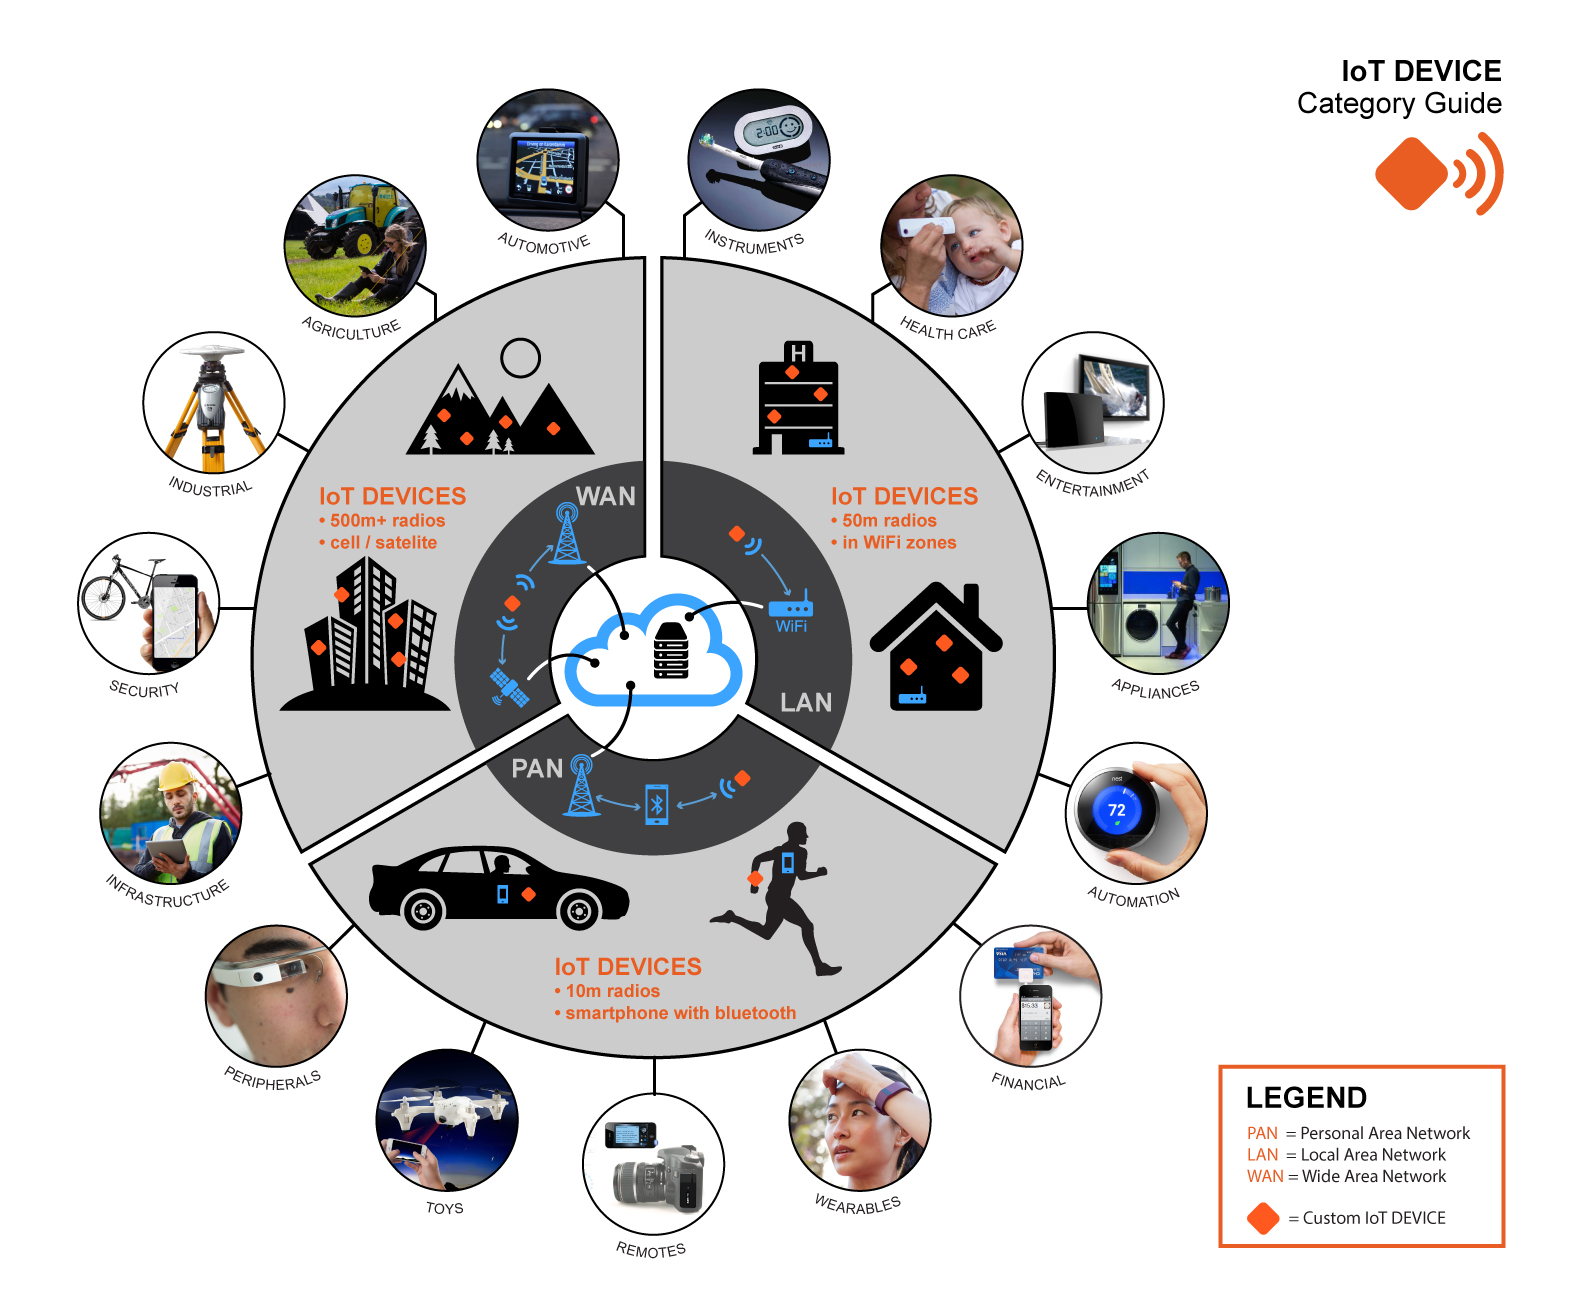
\includegraphics[scale=0.12]{IoT1}
	\caption{IoT devices}
	\label{fig:iot1}
\end{figure}
\end{frame}
\subsection{Cloud computing}
\begin{frame}
\begin{itemize}
	\item Cloud computing
	\begin{itemize}
		\item<1-> \color{blue} {cloud offers various benefits such as
			scalability and elasticity}
		\item<2-> {consolidation and centralization
			lead to many network hops}
		\item<3-> \color{red}{results in high latencies and high bandwidth consumption}
		
	\end{itemize}
\end{itemize}
\begin{figure}
	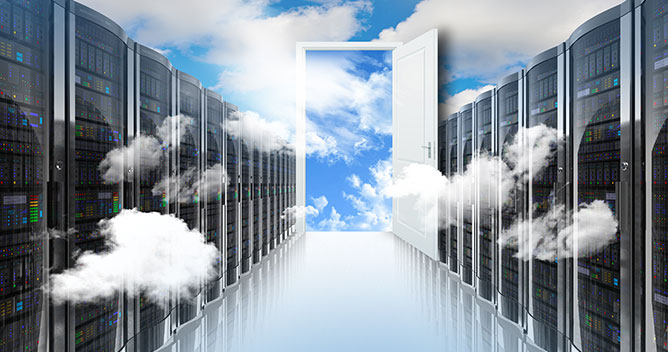
\includegraphics[scale=0.35]{cloud-computing-2}
	\caption{Cloud computing}
	\label{fig:cloud-computing-2}
\end{figure}
\end{frame}
\begin{frame}
\begin{itemize}
	\item Healthcare
\end{itemize}	
\begin{figure}
	\centering
	
\includegraphics[width=0.7\linewidth]{healthcare}
	\caption{Healthcare}
	\label{fig:healthcare}
\end{figure}
\end{frame}
\begin{frame}
\begin{itemize}
	\item Augmented reality
\end{itemize}	
\begin{figure}
	\centering
	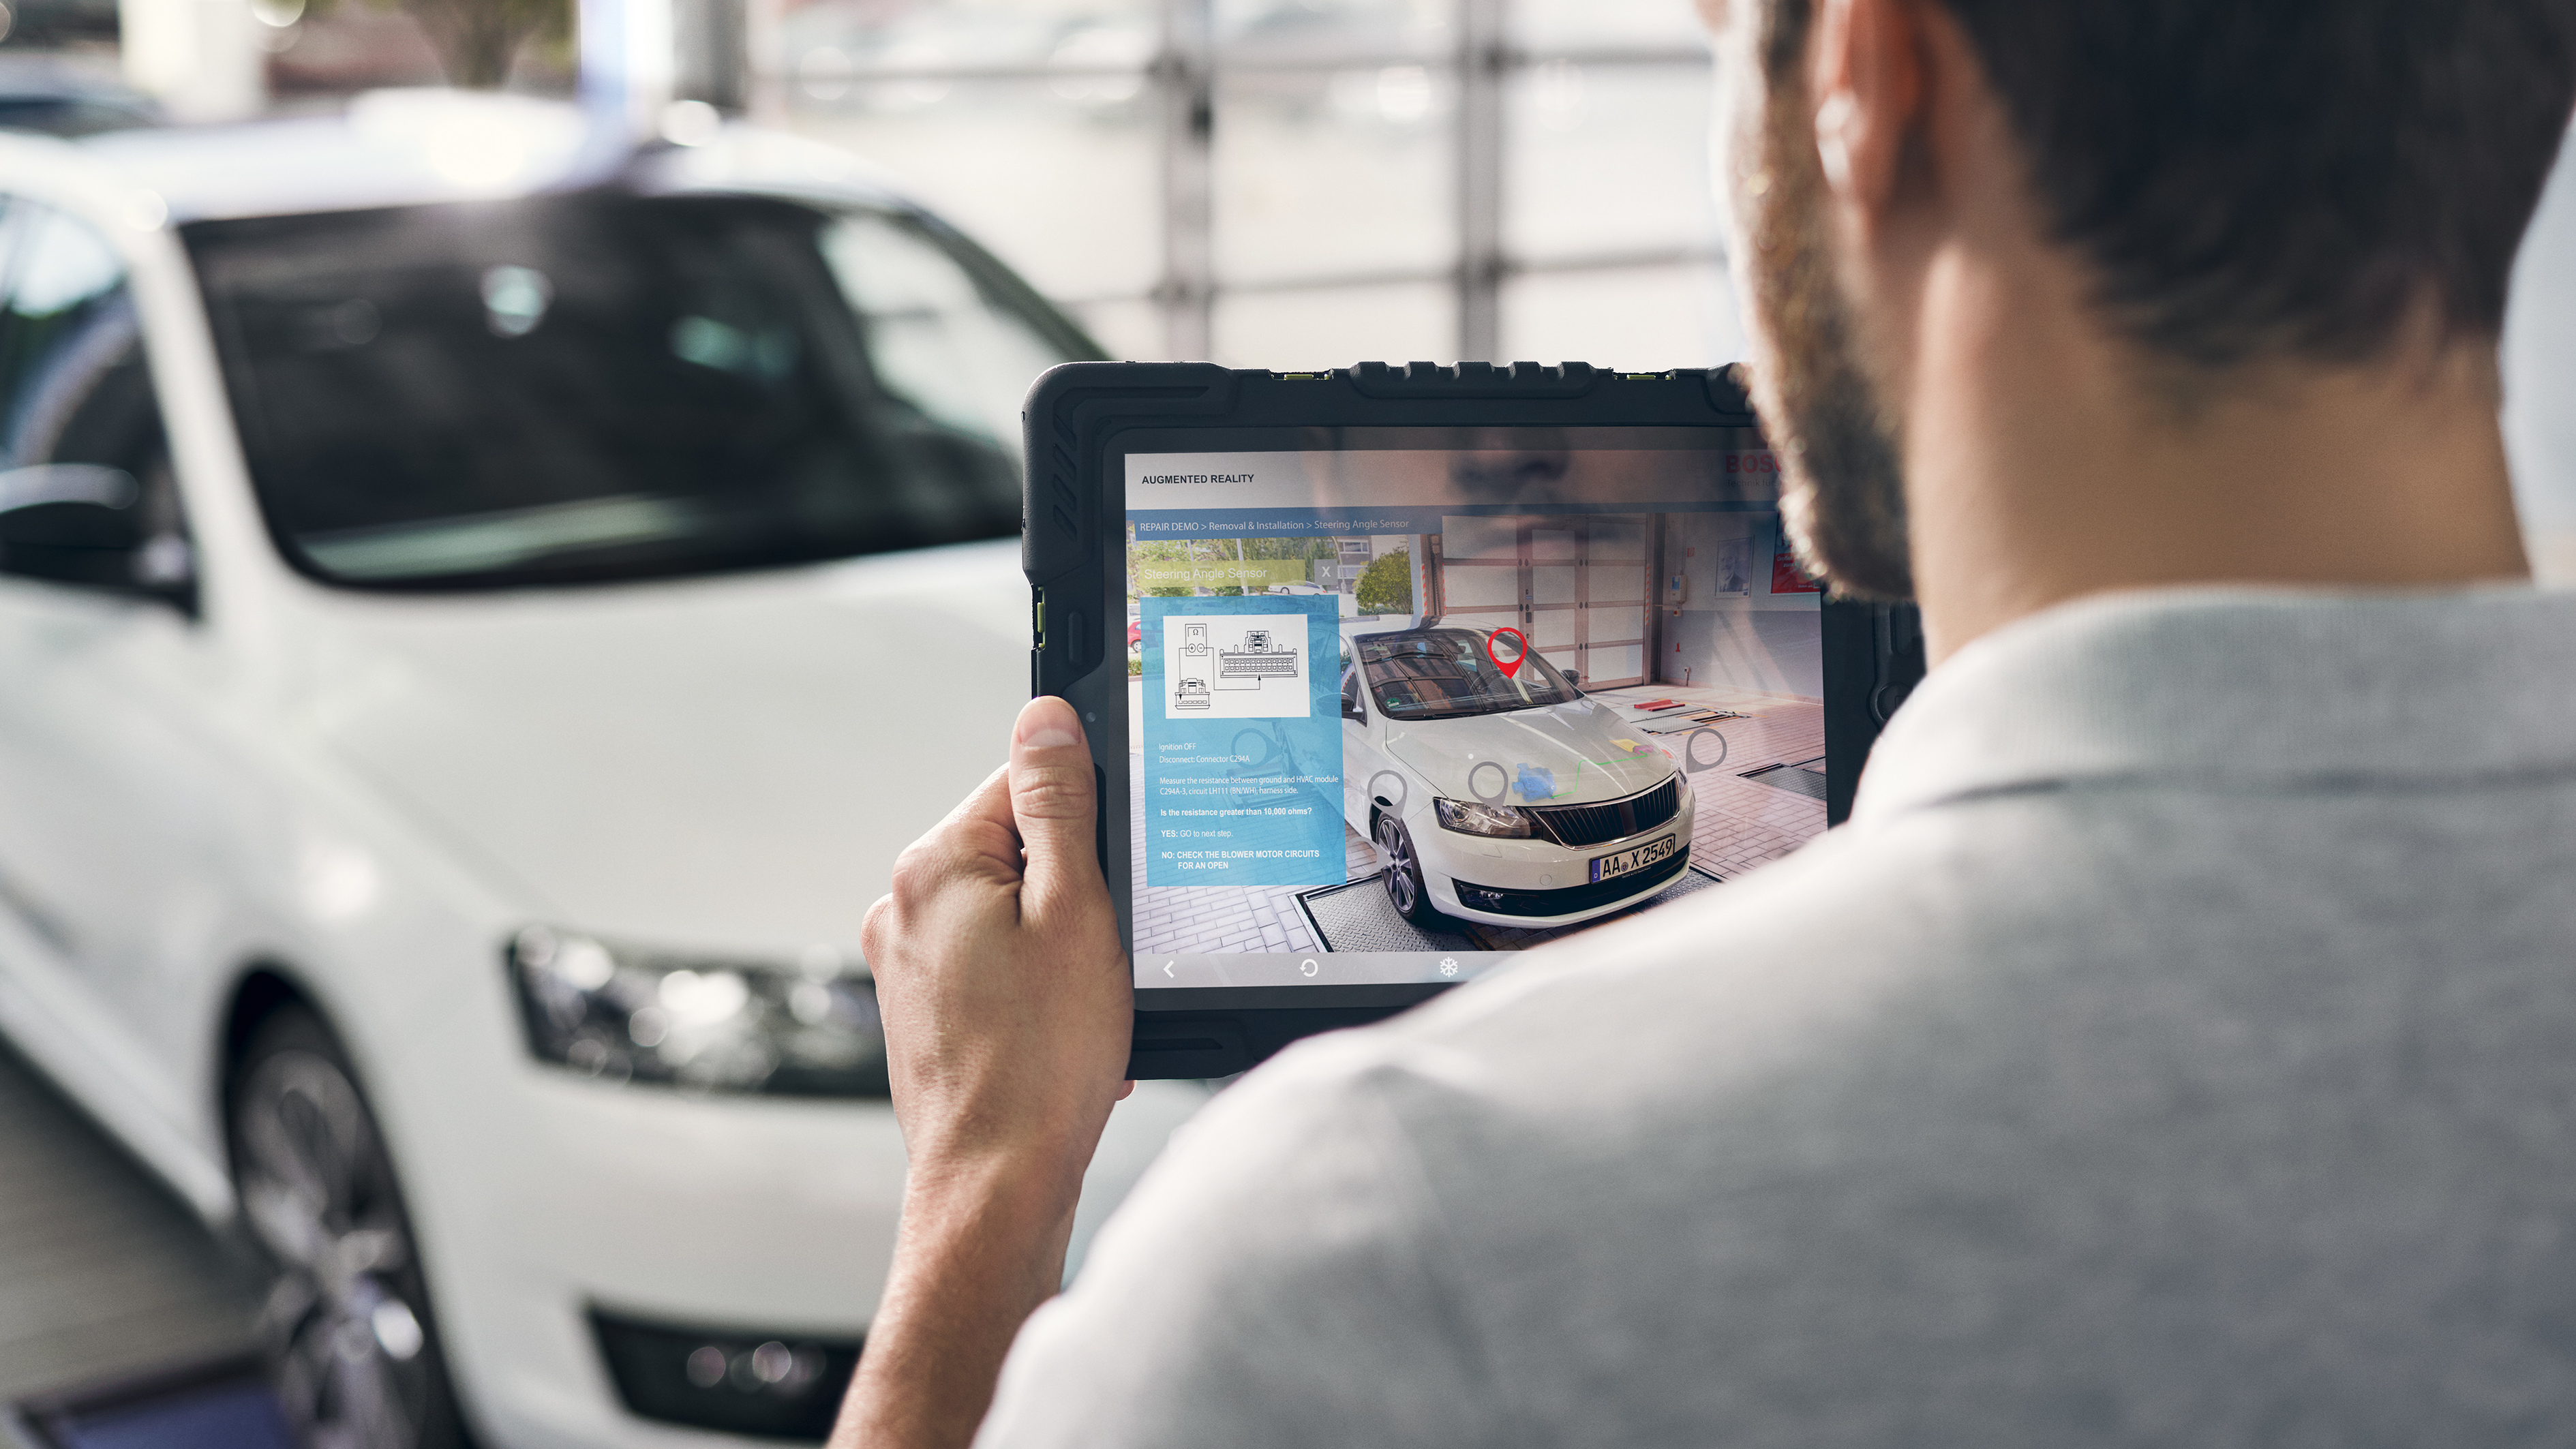
\includegraphics[width=0.7\linewidth]{agmented_R}
	\caption{Augmented reality}
	\label{fig:agmentedr}
\end{figure}
\end{frame}
\subsection{Fog computing}
\begin{frame}
	\begin{itemize}
		\item Fog computing
		\begin{itemize}
			\item<1-> {offers distributed
				edge cloud close to the Things}
		\end{itemize}
	\end{itemize}
\begin{figure}
	\centering
	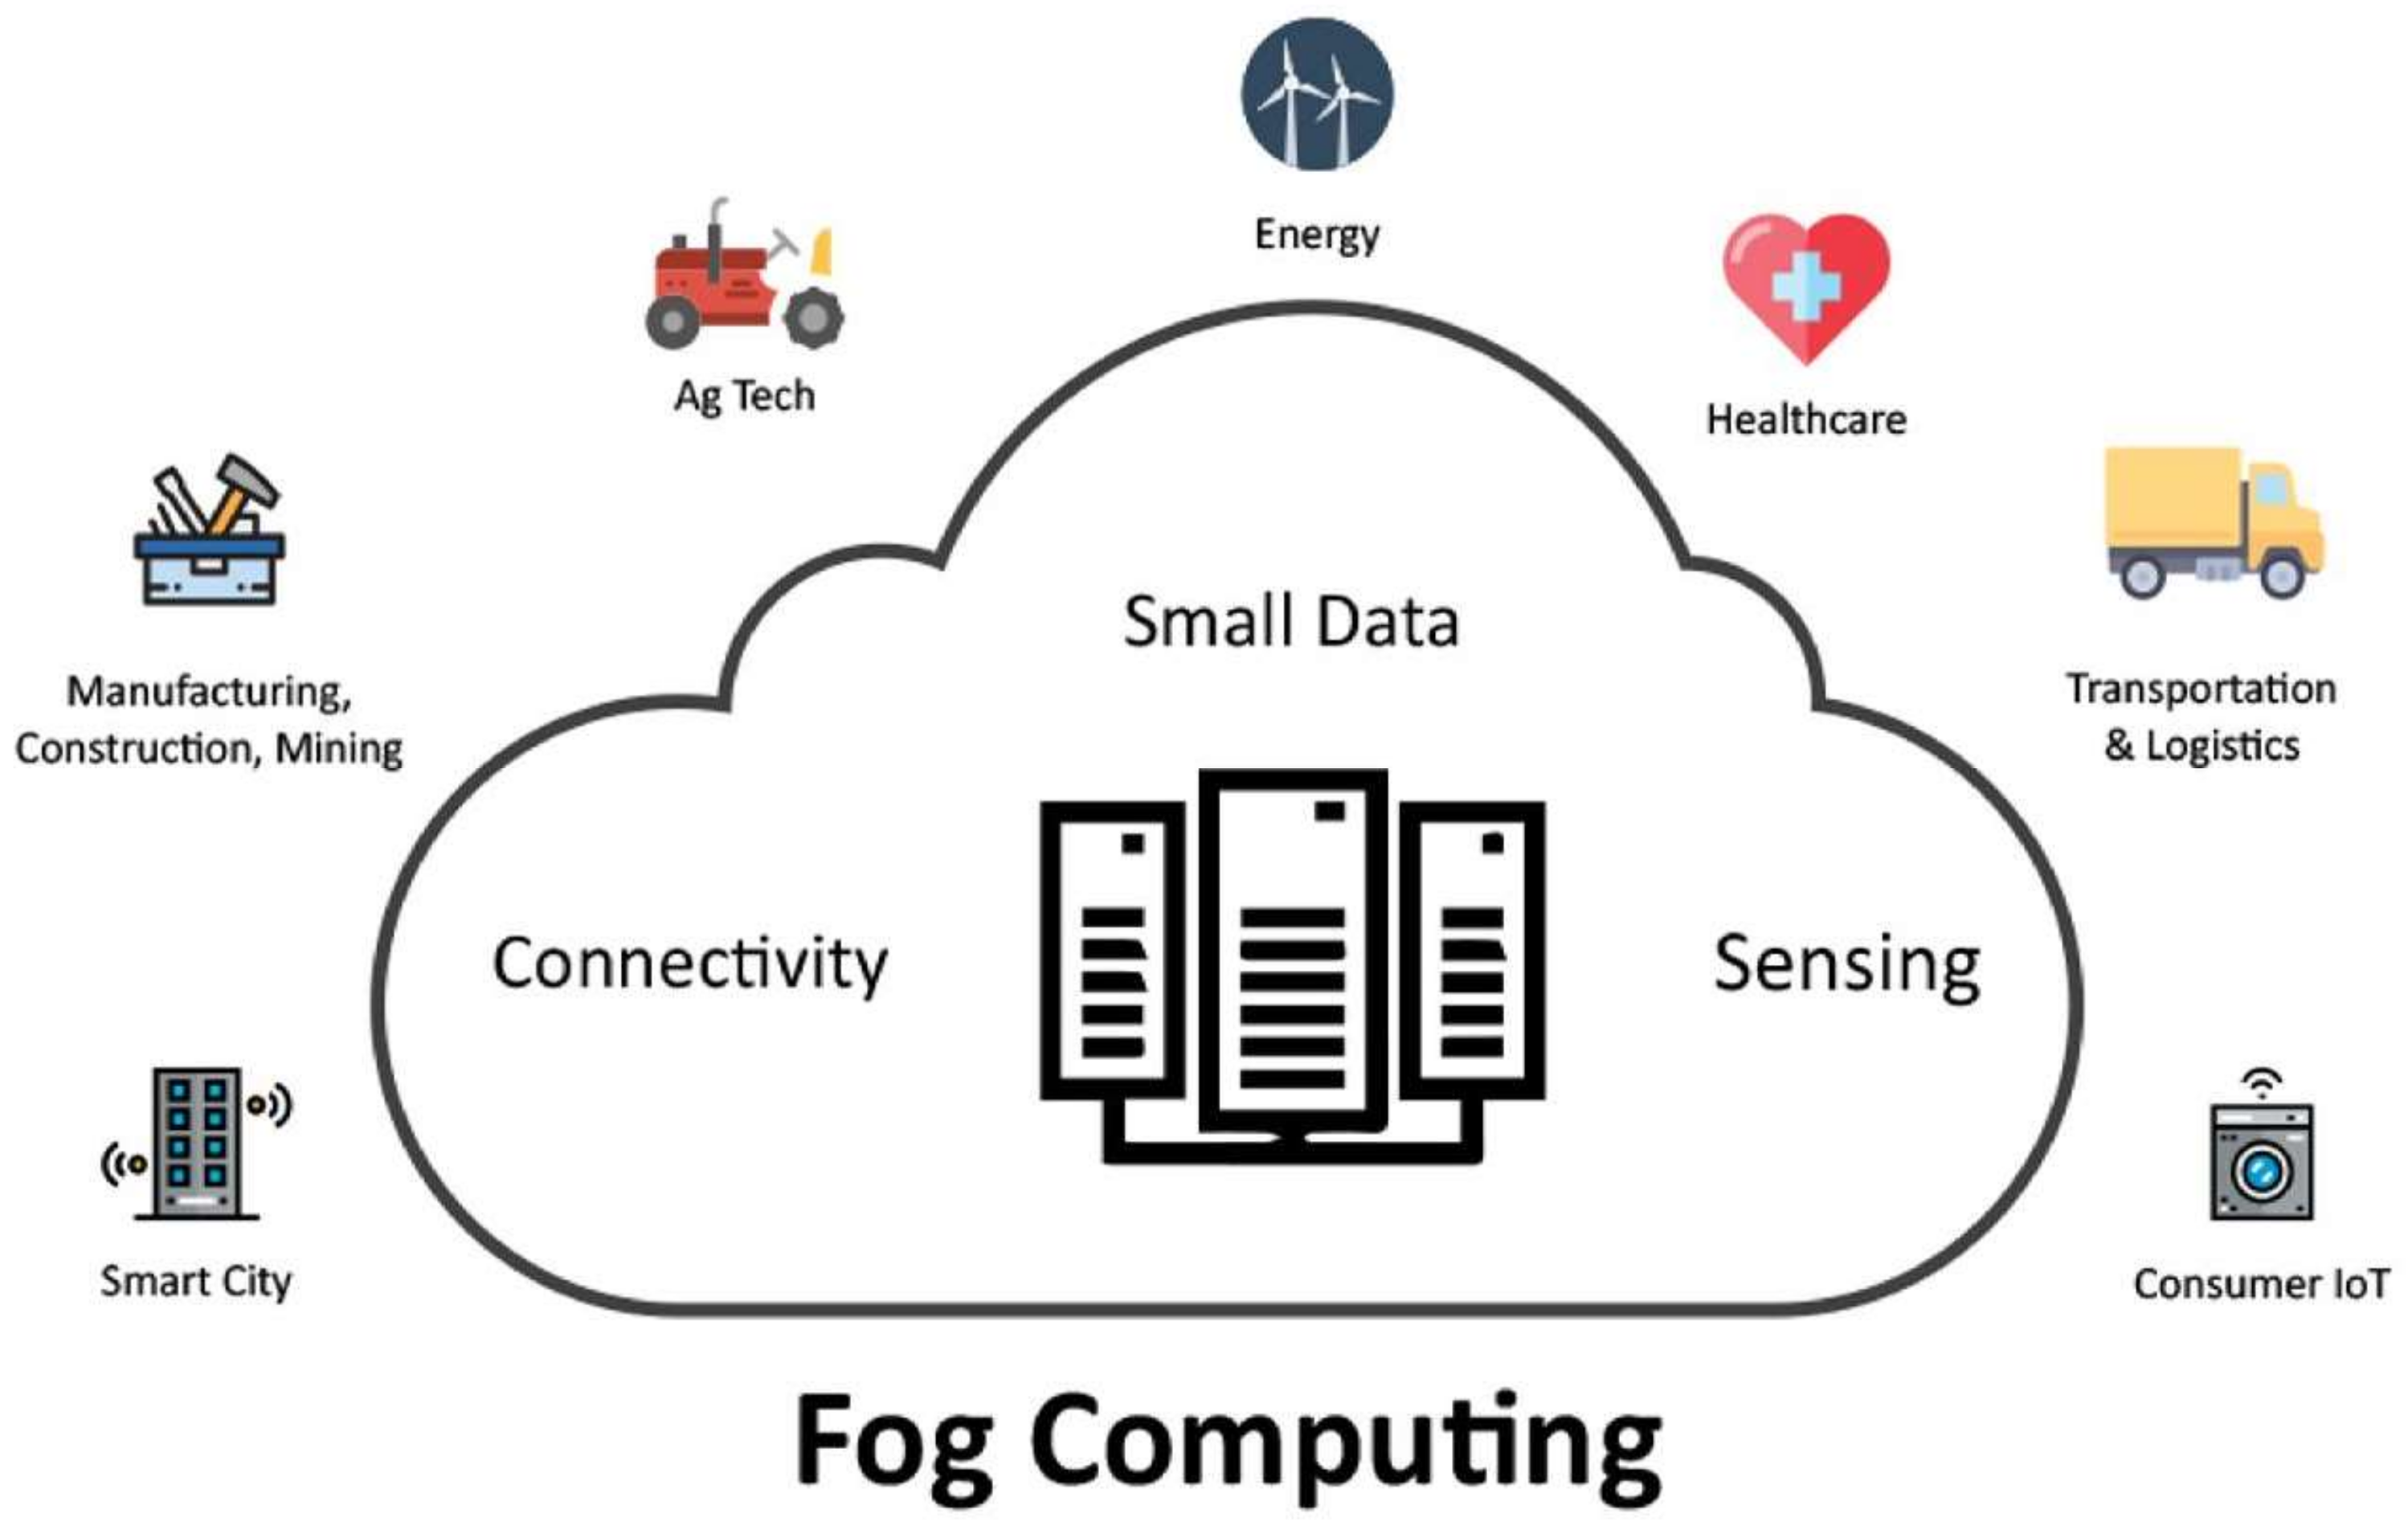
\includegraphics[width=0.7\linewidth]{fog-computing}
	\label{fig:fog-computing}
\end{figure}

\end{frame}
\subsection[Fog-to-Cloud]{Fog-to-Cloud computing system}
\begin{frame}
	\begin{itemize}
	\item Fog-to-Cloud computing system
	\begin{itemize}
		\item<1-> {fog and cloud work together}
		\item<2-> {provide computing, storage, and application servicesin the IoT domain}
		\item<3-> \color{red}{complex management of such a
			network of distributed fogs}
			
	\end{itemize}
\end{itemize}
\begin{figure}
	\centering
	\includegraphics[scale=0.13]{"Fog-to-cloud computing system"}
	\caption{Fog-to-Cloud computing system}
	\label{fig:fog-to-cloud-computing-system}
\end{figure}
\end{frame}
\subsection[SDN and NFV]{Software Defined Network and network function virtualization}
\begin{frame}
	\begin{itemize}
		\item Software Defined Network(SDN)
		\begin{itemize}
			\item<1-> {SDN separates the control and data planes}
		\end{itemize}
	\end{itemize}
\begin{figure}
	\centering
	
\includegraphics[width=0.7\linewidth]{sdn2}
	\caption{Software Defined Network}
	\label{fig:sdn2}
\end{figure}

\end{frame}	
\begin{frame}
\begin{itemize}
	\item network function virtualization(NFV)
	\begin{itemize}
		\item<1-> {NFV reshapes dedicated hardware functionality}
		\item<2-> {software modules named virtual network functions (VNFs)}
		\item<3-> \color{blue}{agile and scalable service placement}
		\item <4-> \color{blue} {reducing Capital
			Expenditure (CAPEX) and Operation Expense (OPEX)}
	\end{itemize}
\end{itemize}
\begin{figure}
	\centering
	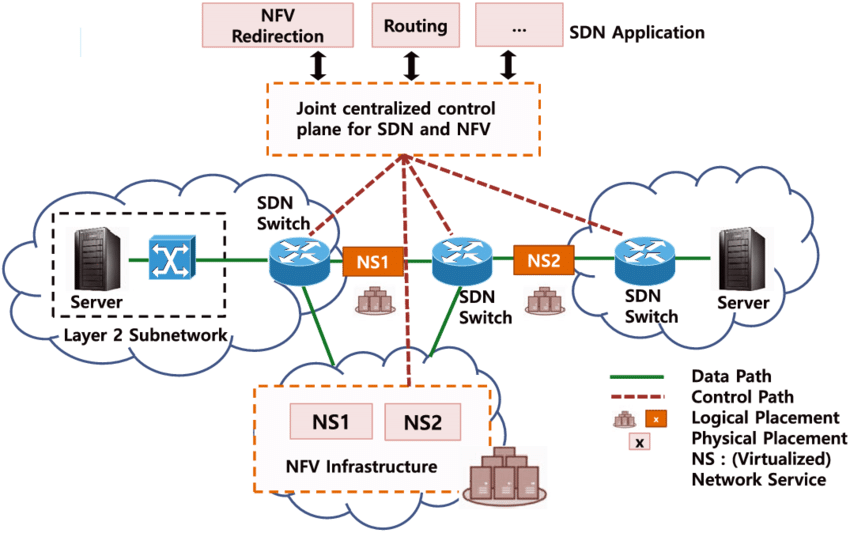
\includegraphics[width=0.62\linewidth]{Architecture-of-a-software-based-network-with-support-for-network-virtualization-NFV}
	\caption{SDN based network with support for NFV}
	\label{fig:architecture-of-a-software-based-network-with-support-for-network-virtualization-nfv}
\end{figure}
\end{frame}
\begin{frame}
	\begin{itemize}
		\item {Service Function Chaining(SFC)}	
		\begin{itemize}
			\item <1->{specific set of VNFs}
			\item <2->{joint VNF placement and traffic routing
				are called SFC mapping}	
		\end{itemize}
	\end{itemize}
\begin{figure}
	\centering
	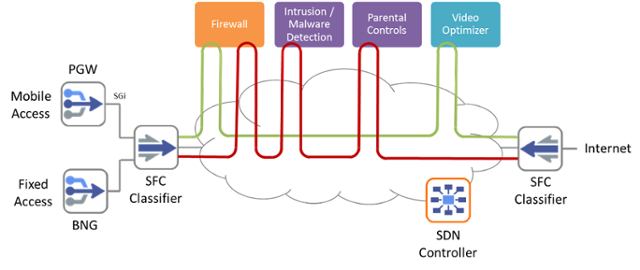
\includegraphics[width=0.9\linewidth]{sfcexample}
	\caption{Service Function Chaining}
	\label{fig:sfcexample}
\end{figure}
\end{frame}
\subsection{Related Work}
\begin{frame}
	\begin{table}
		\begin{tabular}{|c|c|c|c|c|}
			\toprule
			\textbf{Author} & \textbf{Year} & \textbf{Mapping} &\textbf{Solution}& \textbf{Objective}\\
			\midrule
			Draxler & 2017 & VNFs mapping & heuristic & total data rate \\
			 & & & and exact & and total latency\\
			 \hline
			 Huin &2018 & Placement& exact &total latency\\
             \hline
             Masri&2017& Select optimal  &exact &total latency\\
              & & fog or cloud& & \\
             \hline
             Fan&2017&Task scheduling & heuristic & maximizing the  \\
              & &in a fog-to-cloud & &profits of fog  \\
               & & computing system & & service provider \\
               \hline
               Gupta& 2017& VNFs mapping & ILP  & bandwidth \\
               & & & column&consumption\\
               & & & -generation& \\
               & & &based model &\\
			\bottomrule
		\end{tabular}
		\caption{Related Work}
	\end{table}
	
\end{frame}
\begin{frame}
\begin{itemize}{}	
	\item <1-> { do not
		consider SFC mapping in the F2C architecture which is critical in the IoT domain}
	\item <2-> {do not consider the Service Level Agreement(SLA) as a constraint, while in our formulation it is considered}
	\item <3-> {we propose an ILP solution that provides the
		exact solution for SFC mapping in the F2C architecture}
	\item <4-> {in order to minimize total latency of network}
	\begin{itemize}
		\item <5-> {the
			number of instances for each SFC and replicas for each VNF are
			considered}
	\end{itemize}
\end{itemize}
\end{frame}
\section{System Model}
\subsection{Problem statement}
\begin{frame}
\begin{itemize}
	\item <1-> {Problem statement}
\begin{itemize}
	\item <1-> {network topology}
	\item <2-> {capacity and latency of links}
	\item <3-> {computing resources at the fogs and cloud nodes}
	\item <4-> {traffic
		flows between two pairs of fog or fogs and cloud requiring a
		specific SFC}
	\item <5-> {users’ SLA}	
	\item <6-> {instances’ number}
	\item <7-> \color{blue}{placement of VNFs}
	\item <8-> \color{blue}{corresponding traffic routing}
	\item <9-> \color{blue}{users’
		assignment to the SFC instances}
	\item <10-> \color{red}{minimize overall latency of
		network}
\end{itemize}
\end{itemize}
\begin{figure}	
	
\includegraphics[width=0.3\linewidth]{problem_bullseye}
	\label{fig:problembullseye}
\end{figure}
\end{frame}

\subsection{Modeling}
\begin{frame}
	\begin{itemize}
		\item <1-> {Service Function Chaining (SFC)
	\begin{equation}
	[SFC\: c]\quad f_{\sigma_{1}(c)} \to f_{\sigma_{2}(c)} \to \dots \to f_{\sigma_{n_c}(c)}
	\end{equation}}
		\item <2-> {generate all configurations of each SFC $c$  $\to$ $\hat{\Gamma}_c$}
		\item <3-> {aggregation of all configuration of SFCs $\to$ $\hat{\Gamma}$}
		\item <4-> {Each configuration ($\hat{\gamma}$) of SFC c is characterized by:}
		\begin{itemize}
			\item <4-> {Location of VNFs $\to$ $a^{\hat{\gamma}}_{vi}$}
		\end{itemize}
	\end{itemize}
		
\end{frame}
\subsection{Objective function}

\subsection{Constrants}

\section{Numeric Results}
\begin{frame}
\frametitle{Paragraphs of Text}

\end{frame}

%------------------------------------------------

\begin{frame}
\frametitle{Bullet Points}
\begin{itemize}
\item Lorem ipsum dolor sit amet, consectetur adipiscing elit
\item Aliquam blandit faucibus nisi, sit amet dapibus enim tempus eu
\item Nulla commodo, erat quis gravida posuere, elit lacus lobortis est, quis porttitor odio mauris at libero
\item Nam cursus est eget velit posuere pellentesque
\item Vestibulum faucibus velit a augue condimentum quis convallis nulla gravida
\end{itemize}
\end{frame}

%------------------------------------------------

\begin{frame}
\frametitle{Blocks of Highlighted Text}
\begin{block}{Block 1}
Lorem ipsum dolor sit amet, consectetur adipiscing elit. Integer lectus nisl, ultricies in feugiat rutrum, porttitor sit amet augue. Aliquam ut tortor mauris. Sed volutpat ante purus, quis accumsan dolor.
\end{block}

\begin{block}{Block 2}
Pellentesque sed tellus purus. Class aptent taciti sociosqu ad litora torquent per conubia nostra, per inceptos himenaeos. Vestibulum quis magna at risus dictum tempor eu vitae velit.
\end{block}

\begin{block}{Block 3}
Suspendisse tincidunt sagittis gravida. Curabitur condimentum, enim sed venenatis rutrum, ipsum neque consectetur orci, sed blandit justo nisi ac lacus.
\end{block}
\end{frame}

%------------------------------------------------

\begin{frame}
\frametitle{Multiple Columns}
\begin{columns}[c] % The "c" option specifies centered vertical alignment while the "t" option is used for top vertical alignment

\column{.45\textwidth} % Left column and width
\textbf{Heading}
\begin{enumerate}
\item Statement
\item Explanation
\item Example
\end{enumerate}

\column{.5\textwidth} % Right column and width
Lorem ipsum dolor sit amet, consectetur adipiscing elit. Integer lectus nisl, ultricies in feugiat rutrum, porttitor sit amet augue. Aliquam ut tortor mauris. Sed volutpat ante purus, quis accumsan dolor.

\end{columns}
\end{frame}

%------------------------------------------------
\section{Second Section}
%------------------------------------------------

\begin{frame}
\frametitle{Table}
\begin{table}
\begin{tabular}{l l l}
\toprule
\textbf{Treatments} & \textbf{Response 1} & \textbf{Response 2}\\
\midrule
Treatment 1 & 0.0003262 & 0.562 \\
Treatment 2 & 0.0015681 & 0.910 \\
Treatment 3 & 0.0009271 & 0.296 \\
\bottomrule
\end{tabular}
\caption{Table caption}
\end{table}
\end{frame}

%------------------------------------------------

\begin{frame}
\frametitle{Theorem}
\begin{theorem}[Mass--energy equivalence]
$E = mc^2$
\end{theorem}
\end{frame}

%------------------------------------------------

\begin{frame}[fragile] % Need to use the fragile option when verbatim is used in the slide
\frametitle{Verbatim}
\begin{example}[Theorem Slide Code]
\begin{verbatim}
\begin{frame}
\frametitle{Theorem}
\begin{theorem}[Mass--energy equivalence]
$E = mc^2$
\end{theorem}
\end{frame}\end{verbatim}
\end{example}
\end{frame}

%------------------------------------------------

\begin{frame}
\frametitle{Figure}
Uncomment the code on this slide to include your own image from the same directory as the template .TeX file.
%\begin{figure}
%\includegraphics[width=0.8\linewidth]{test}
%\end{figure}
\end{frame}

%------------------------------------------------

\begin{frame}[fragile] % Need to use the fragile option when verbatim is used in the slide
\frametitle{Citation}
An example of the \verb|\cite| command to cite within the presentation:\\~

This statement requires citation \cite{p1}.
\end{frame}

%------------------------------------------------

\begin{frame}
\frametitle{References}
\footnotesize{
\begin{thebibliography}{99} % Beamer does not support BibTeX so references must be inserted manually as below
\bibitem[Smith, 2012]{p1} John Smith (2012)
\newblock Title of the publication
\newblock \emph{Journal Name} 12(3), 45 -- 678.
\end{thebibliography}
}
\end{frame}

%------------------------------------------------

\begin{frame}
\Huge{\centerline{The End}}
\end{frame}

%----------------------------------------------------------------------------------------

\end{document} 